\documentclass[a4paper, 12pt]{article}
\usepackage{pgfplots, mathtools}

%% Listings With Code-Styling and Grey Background
\usepackage{float, listings} 
\lstset{						% Global Listing settings
	language=Verilog,
	numbers=left,
	numberstyle=\tiny\color{gray},
%	firstnumber=1,
	numberfirstline=true,
	stepnumber=1,
	tabsize=2,
	breaklines=true,
}
\usepackage{xcolor, mdframed, graphicx}
\definecolor{code-gray}{gray}{0.93}

%% Make specific pages landscale for larger figures
\usepackage{pdflscape}

%% Custom FSM's
\usepackage{tikz}
\usetikzlibrary{automata, positioning, arrows, positioning}
\tikzset{very thick, ->, >=stealth', node distance=6cm, every state/.style={thick, fill=gray!10}, initial text=$ $}

%% Automatic Word Formatting
\usepackage{xspace}
\newcommand*{\Vivado}{\textit{Vivado}\xspace} % Italicize Vivado
\newcommand*{\SV}{\textbf{SystemVerilog}\xspace} % Bold SystemVerilog

%% Clickable links in the output PDF
\usepackage{hyperref}
\hypersetup{colorlinks=true, linktoc=all, linkcolor=black}

%% Figure Numbering Within Sections
\let\counterwithout\relax
\let\counterwithin\relax
\usepackage{chngcntr}
\counterwithin{figure}{section}

%% Macros for logic timing diagrams
\newcounter{wavenum}
\setlength{\unitlength}{1cm}
% advance clock one cycle, not to be called directly
\newcommand*{\clki}{
  \draw (t_cur) -- ++(0,.3) -- ++(.5,0) -- ++(0,-.6) -- ++(.5,0) -- ++(0,.3)
    node[time] (t_cur) {};
}
\newcommand*{\bitvector}[3]{
  \draw[fill=#3] (t_cur) -- ++( .1, .3) -- ++(#2-.2,0) -- ++(.1, -.3)
                         -- ++(-.1,-.3) -- ++(.2-#2,0) -- cycle;
  \path (t_cur) -- node[anchor=mid] {#1} ++(#2,0) node[time] (t_cur) {};
}
% \known{val}{length}
\newcommand*{\known}[2]{
    \bitvector{#1}{#2}{white}
}
% \unknown{length}
\newcommand*{\unknown}[2][XXX]{
    \bitvector{#1}{#2}{black!20}
}
% \bit{1 or 0}{length}
\newcommand*{\bit}[2]{
  \draw (t_cur) -- ++(0,.6*#1-.3) -- ++(#2,0) -- ++(0,.3-.6*#1)
    node[time] (t_cur) {};
}
% \unknownbit{length}
\newcommand*{\unknownbit}[1]{
  \draw[ultra thick,black!50] (t_cur) -- ++(#1,0) node[time] (t_cur) {};
}
% \nextwave{name}
\newcommand{\nextwave}[1]{
  \path (0,\value{wavenum}) node[left] {#1} node[time] (t_cur) {};
  \addtocounter{wavenum}{-1}
}
% \clk{name}{period}
\newcommand{\clk}[2]{
    \nextwave{#1}
    \FPeval{\res}{(\wavewidth+1)/#2}
    \FPeval{\reshalf}{#2/2}
    \foreach \t in {1,2,...,\res}{
        \bit{\reshalf}{1}
        \bit{\reshalf}{0}
    }
}

% \begin{wave}[clkname]{num_waves}{clock_cycles}
\newenvironment{wave}[3][clk]{
  \begin{tikzpicture}[draw=black, yscale=.7,xscale=1]
    \tikzstyle{time}=[coordinate]
    \setlength{\unitlength}{1cm}
    \def\wavewidth{#3}
    \setcounter{wavenum}{0}
    \nextwave{#1}
    \foreach \t in {0,1,...,\wavewidth}{
      \draw[dotted] (t_cur) +(0,.5) node[above] {t=\t} -- ++(0,.4-#2);
      \clki
    }
}{\end{tikzpicture}}

%$ Specific Line Breaks
% See https://tex.stackexchange.com/questions/26174/ for details
\usepackage[british]{babel} 

%% Page Margins
\usepackage[margin=1.00in]{geometry}

%% Beginning of Document
\begin{document}
\counterwithin{lstlisting}{section} % Listings are numbered within sections
% Title
\title{ECE 440 - Project \#4}
\author{Collin Heist}
\date{\today}
\maketitle

% Table of Content and Listings
\pagenumbering{roman}
\tableofcontents
\renewcommand{\listfigurename}{Figures}
\listoffigures
\lstlistoflistings
\newpage
\pagenumbering{arabic}

% Beginning of Report
\section{Design}
There was really no design consideration necessary for this project. The general circuit was provided to us, and the only interesting component was the instantiation and creation of the memory unit.

For the memory unit, I utilized the distributed memory generator with a 4-bit address, and a two-bit input and output bus. However, because the address inputs on the larger circuit diagram is only 2-bit. This tripped me up at first, as my simulation was showing indeterminate values (of course) and I didn't realize why. This was resolved by wiring the address input with two zeros appended. The isolated register was simple enough, and was within a synchronized block that updated the output signal with the results of the memory unit. The rest of the circuit implementation was as expected.

Initializing the memory was done using a \textbf{.coe} file, which is shown in \textbf{Listing~\ref{lst:coe-file}}.

\begin{landscape}
\section{Simulations}
\subsection{Behavioral Simulation}
The results of my behavioral and post-synthesis simulations are exactly identical. The behavioral simulation has the benefit of showing internal signals, which I've partitioned into inputs, those of the memory module, and the output signals.

\begin{figure}[H]
\centering
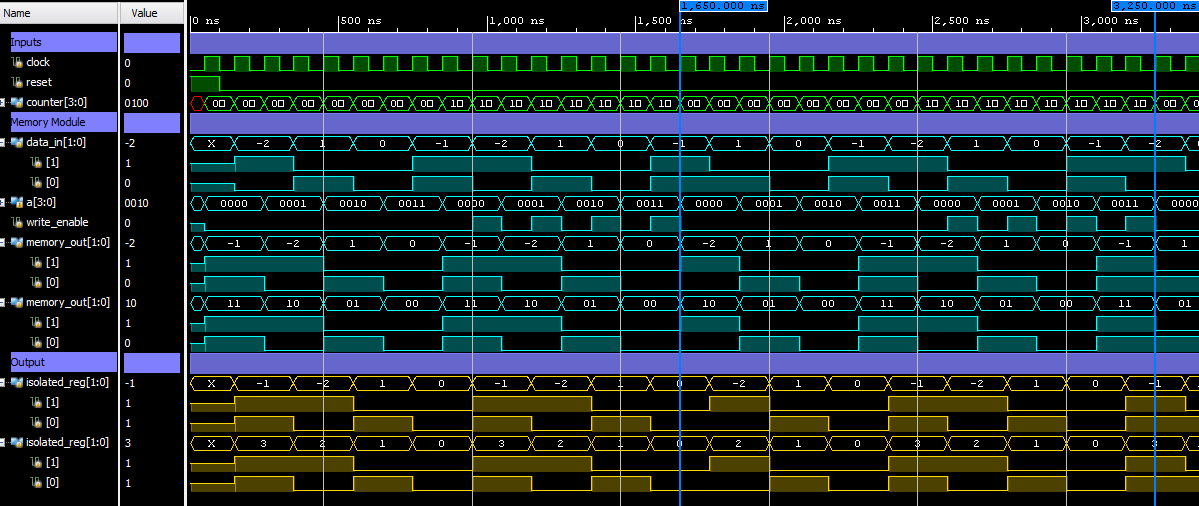
\includegraphics[width=0.85\paperheight, keepaspectratio=true]{Sources/Behav-Sim-Small-1.PNG}
\caption{First Section of the Behavioral Simulation.}
\label{fig:behav-sim}
\end{figure}

\begin{figure}[H]
\centering
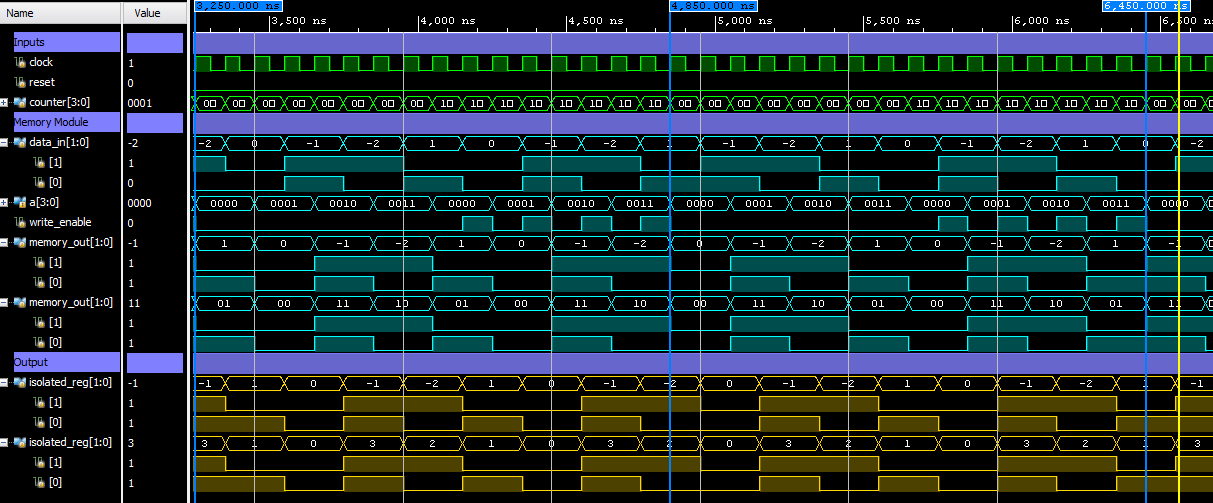
\includegraphics[width=0.85\paperheight, keepaspectratio=true]{Sources/Behav-Sim-Small-2.PNG}
\caption{Second Section of the Behavioral Simulation.}
\label{fig:behav-sim}
\end{figure}

\subsection{Post-Synthesis Timing Simulation}
Showing only the primary inputs and outputs, the identical output data patterns can be seen. Memory accesses occur in an identical pattern, as the counter is initialized to 0, incremented by the clock, and thus is not variable in any way.

\begin{figure}[H]
\centering
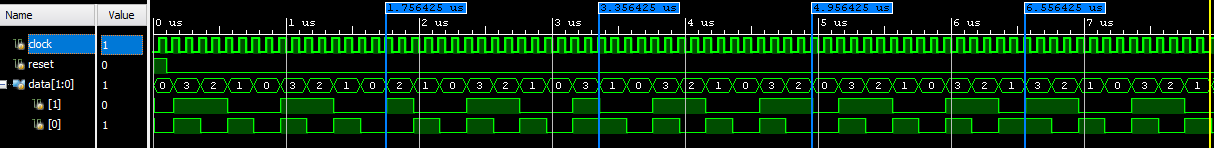
\includegraphics[width=0.80\paperheight, keepaspectratio=true]{Sources/Post-Synth-Sim.PNG}
\caption{Post-Synthesis Timing Simulation.}
\label{fig:post-synth-sim}
\end{figure}
\end{landscape}

\section{Source Code}
\begin{mdframed}[backgroundcolor=code-gray, roundcorner=10pt, innerleftmargin=25, innertopmargin=5, innerbottommargin=5]	
\lstinputlisting[caption=\textit{Weird Circuit} Module, label={lst:wrapper}]{Sources/weird_circuit.sv}
\end{mdframed}

\begin{mdframed}[backgroundcolor=code-gray, roundcorner=10pt, innerleftmargin=25, innertopmargin=5, innerbottommargin=5]	
\lstinputlisting[caption=Testbench, label={lst:testbench}]{Sources/testbench.sv}
\end{mdframed}

\begin{mdframed}[backgroundcolor=code-gray, roundcorner=10pt, innerleftmargin=25, innertopmargin=5, innerbottommargin=5]	
\begin{lstlisting}[caption=Memory Initialization File, label={lst:coe-file}]
memory_initialization_radix = 2;
memory_initialization_vector = 11 10 01 00;
\end{lstlisting}
\end{mdframed}

\end{document}